\documentclass[10pt,french]{report}
\usepackage{etex}
\usepackage[utf8]{inputenc}
\usepackage[T1]{fontenc}
\usepackage{tikz}
\usetikzlibrary{calc,arrows,intersections}
\usepackage{mathtools,amsmath}
\usepackage{babel}
\DecimalMathComma

\begin{document}
\begin{center}
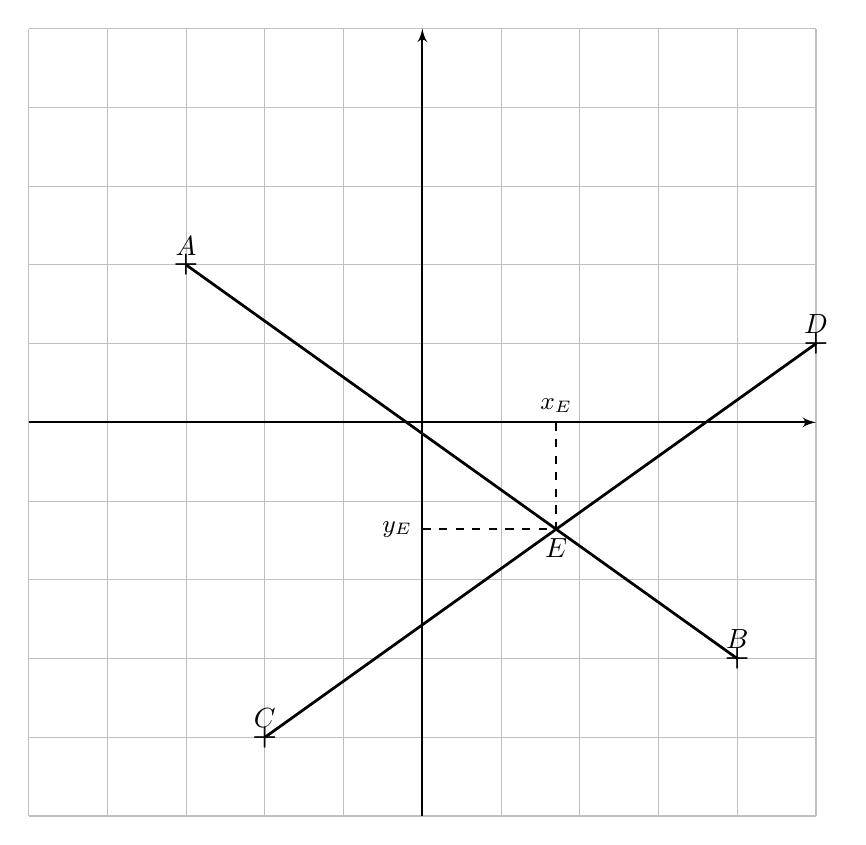
\begin{tikzpicture}[>=latex']
\def\xmin{-5}\def\xmax{5}\def\ymin{-5}\def\ymax{5}
\draw[lightgray] (\xmin,\ymin) grid (\xmax,\ymax);
\draw[->, line width = 0.7pt] (\xmin,0)--(\xmax,0);
\draw[->, line width = 0.7pt] (0,\ymin)--(0,\ymax);
\coordinate (A) at (-3,2);
\draw (A) node{\textbf +} node[above] {$A$};
\coordinate (B) at (4,-3);
\draw (B) node{\textbf +} node[above] {$B$};
\draw[line width=1pt] (A)--(B);
\coordinate (C) at (-2,-4);
\draw (C) node{\textbf +} node[above] {$C$};
\coordinate (D) at (5,1);
\draw (D) node{\textbf +} node[above] {$D$};
\draw[line width=1pt] (C)--(D);
\coordinate (E) at (intersection of A--B and C--D);
\draw (E) node[below] {$E$};
\draw[dashed, line width=0.7pt]
    let \p1=(E) in
        (\x1,0) node[above] {\small $x_E$}
        |- (0,\y1) node[left] {\small $y_E$};
\end{tikzpicture}
\end{center}

\begin{center}
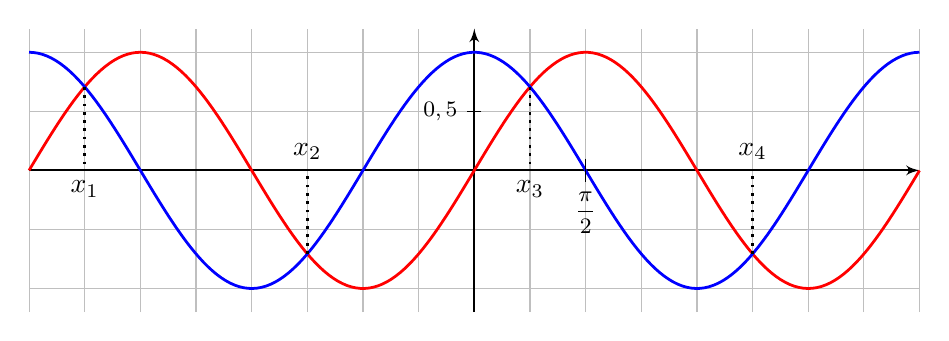
\begin{tikzpicture}[>=latex', x=0.9cm, y=1.5cm]
\def\xmin{-2*pi}\def\xmax{2*pi}\def\ymin{-1.2}\def\ymax{1.2}
\draw[lightgray] (\xmin,\ymin) grid[xstep={pi/4},ystep=0.5] (\xmax,\ymax);
\draw[->, line width = 0.7pt] (\xmin,0)--(\xmax,0);
\draw[->, line width = 0.7pt] (0,\ymin)--(0,\ymax);
\draw[name path=sinus, line width = 1pt, red] plot[samples=200,domain=-2*pi:2*pi] (\x,{sin(\x r)});
\draw[name path=cosinus, line width = 1pt, blue] plot[samples=200,domain=-2*pi:2*pi] (\x,{cos(\x r)});
\draw (pi/2,0.1) -- (pi/2,-0.1) node[below] {\footnotesize $\dfrac\pi2$};
\draw (0.1,0.5) -- (-0.1,0.5) node[left] {\footnotesize $0,5$};
\coordinate[name intersections={of=sinus and cosinus, name=PtInter}];
\foreach \pt in {1,3}
    \draw[dotted, line width=1pt] let \p1=(PtInter-\pt) in (\p1) -- (\x1,0) node[below] {$x_\pt$};
\foreach \pt in {2,4}
    \draw[dotted, line width=1pt] let \p1=(PtInter-\pt) in (\p1) -- (\x1,0) node[above] {$x_\pt$};
\end{tikzpicture}
\end{center}
\end{document}